\chapter{Risultati sperimentali}
\label{cap:risultati}
\thispagestyle{empty}

\begin{quotation}
{\footnotesize
\noindent\emph{Doc: Mani in alto! \\
Macchinista: E' una rapina? \\
Doc: E' un esperimento scientifico! Fermi il treno prima di arrivare al prossimo scambio!}
\begin{flushright}
Ritorno al Futuro, parte III
\end{flushright}
}
\end{quotation}
\vspace{0.5cm}

In questo capitolo descriveremo qualitativamente i risultati sperimentali riguardanti i vari moduli del sistema.

\section{Riconoscimento degli oggetti}
Il riconoscimento degli oggetti è abbastanza robusto rispetto ai falsi positivi, a patto che si utilizzi una knowledge base adatta all'ambiente utilizzato. Il riconoscimento è abbastanza robusto rispetto al rumore presente nell'immagine, il sistema ottenuto quindi è abbastanza preciso. 
Tuttavia, il riconoscimento è fortemente basato sugli output dell'algoritmo di Canny per estrarre i bordi e della trasformata di Hough per le linee. In particolare l'algoritmo di Canny è abbastanza sensibile alle variazioni di luce, ed è possibile non riuscire a estrarre correttamente i bordi dall'immagine, e conseguentemente le linee, se le condizioni di luce sono particolarmente sfavorevoli. Questo problema, unito al fatto che la trasformata di Hough probabilistica non riconosce completamente le linee se il bordo riconosciuto da Canny non è abbastanza pulito, fa sì che il tasso di recupero dell'algoritmo non sia elevatissimo. Questo problema è mitigato dall'uso di euristiche meno restrittive e da una analisi localizzata dell'immagine nell'algoritmo di riconoscimento, ma in alcuni casi potrebbe essere problematico nell'algoritmo di individuazione. 

Un'altra possibile causa di cattiva interpretazione dell'immagine è la deformazione prospettica degli oggetti. Infatti, gli oggetti visti da punti di vista particolarmente angolati sono riconosciuti con un fattore di forma molto più schiacciato rispetto alla realtà, e questo può causare una cattiva interpretazione da parte del reasoner. Si può facilmente eliminare il problema calcolando il vero fattore di forma dell'oggetto visto, supponendo che sia un rettangolo, riconducendosi a una rettificazione metrica. Tuttavia questo processo può essere computazionalmente costoso, e in generale non ci è sembrato necessario al fine di implementare un primo prototipo del sistema.

\begin{figure}[ht]
  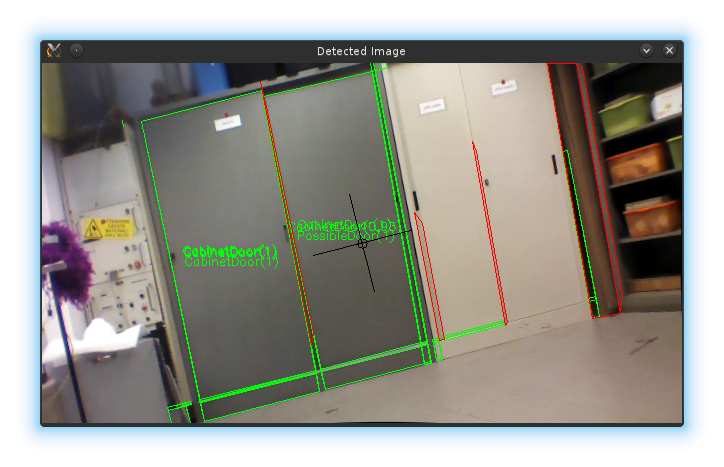
\includegraphics[width=\textwidth]{immagini/risultati/detection}
  \caption[Individuazione degli oggetti]{Individuate le porte dell'armadio}
  \label{fig:detection}
\end{figure}

\begin{figure}[ht]
  \centering
  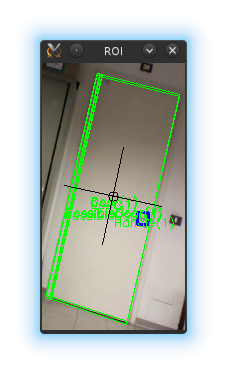
\includegraphics{immagini/risultati/recognition1}
  \caption[Riconoscimento della porta]{Riconosciuta una porta con la sua maniglia}
  \label{fig:recognition1}
\end{figure}

\begin{figure}[ht]
  \centering
  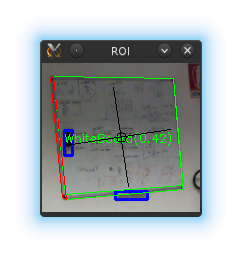
\includegraphics{immagini/risultati/recognition2}
  \caption[Riconoscimento della lavagna]{Riconosciuta la lavagna}
  \label{fig:recognition2}
\end{figure}

\clearpage

\section{Reasoning}
L'algoritmo di reasoning è fortemente dipendente dalla knowledge base implementata. Grazie alla logica fuzzy, se istruito con una knowledge base adatta al contesto, risulta estremamente efficiente e robusto al rumore. Il costo computazionale è estremamente variabile, dipende infatti dal classificatore utilizzato, e dal numero delle istanze da classificare. Se il numero delle istanze è basso, il classificatore riesce a calcolare l'output in tempi dell'ordine di grandezza del millisecondo, su un processore Intel Core i7-4500U.
Se si ha un elevato numero di istanze e si devono gestire relazioni complesse, il tempo di calcolo può essere nell'ordine delle centinaia di millisecondi, o più, se il numero di istanze fosse maggiore a quelle normalmente considerate nei nostri test (nell'ordine delle decine o centinaia).
In generale, il problema dell'algoritmo di reasoning è la natura combinatoria dell'algoritmo utilizzato per risolvere le dipendenze cicliche, in cui è necessario testare ogni possibile combinazione di candidati delle classi considerate. Questo problema può essere risolto in vari modi: 
\begin{itemize}
 \item Restringendo il numero di istanze da classificare simultaneamente a priori, passando solo le istanze correlate all'algoritmo di reasoning.
 \item Scrivendo classificatori intelligenti, in grado di discriminare feature su più livelli della gerarchia, riducendo il numero di candidati che appartengono alle classi coinvolte nelle dipendenze cicliche.
 \item Implementando all'interno del reasoner degli indici di feature basati sui descrittori coinvolti nelle relazioni cicliche, in modo da poter compiere una ricerca basata sul loro valore.
\end{itemize}
Ci è sembrato che le prime due soluzioni fossero più pratiche e semplici da seguire, e quindi le abbiamo implementate nel nostro sistema, lasciando a futuri sviluppi la proposta dell'indicizzazione.

\clearpage

\section{Tracking}
L'algoritmo di tracking usato ha prestazioni estremamente buone. Il tasso di recupero dell'algoritmo è maggiore del 90\%, anche se questo dipende parzialmente dalle caratteristiche dell'oggetto seguito. Il bounding box disegnato non è tuttavia sempre e comunque preciso, soprattutto quando si tratta di seguire oggetti da posizione angolate, dove la deformazione prospettica diventa più significativa. Maggiorando il bounding box, tuttavia, si ottengono risultati buoni anche quando il punto di vista è moderatamente angolato, poiché l'oggetto risulta essere contenuto completamente nel bounding box considerato.

La precisione dell'algoritmo non è altrettanto buona, poiché si possono verificare riconoscimenti errati, soprattutto quando l'oggetto considerato non è nel campo visivo della telecamera. Infatti, poiché l'algoritmo considera una sola istanza possibile dell'oggetto considerato, sarà il vero oggetto a essere riconosciuto.

Per quanto riguarda il costo computazionale, l'algoritmo riesce a lavorare ad elevato frame rate se gli oggetti seguiti simultaneamente sono pochi. Questo quindi può essere un problema quando si devono costruire mappe con molti oggetti. Il problema tuttavia è risolto in maniera abbastanza semplice considerando come track attive solo quelle che potrebbero trovarsi nel campo visivo del robot, anziché tutte le track seguite, ed eventualmente limitando il numero di match cercati nell'immagine a ogni iterazione. Utilizzando la mappa si risolve anche quasi totalmente il problema del riconoscimento errato delle track fuori dall'immagine.
L'ultimo aspetto da considerare dell'algoritmo di tracking implementato è la sua capacità di riconoscere un oggetto già seguito.
Abbiamo notato che l'euristica da noi implementata funziona estremamente bene nella maggior parte dei casi, soffrendo solo qualche problema quando l'algoritmo di tracking, a causa del numero elevato di track, non riesce ad avere un frame rate paragonabile al nodo che individua gli oggetti. In questi casi, l'algoritmo di tracking potrebbe non aver riconosciuto in tempo un oggetto entrato nell'immagine, che invece è stato già individuato, generando una nuova track sull'oggetto. Questo problema tuttavia può essere facilmente risolto a livello di mappa, riuscendo a individuare gli oggetti che occupano lo stesso spazio come equivalenti.

\begin{figure}[ht]
  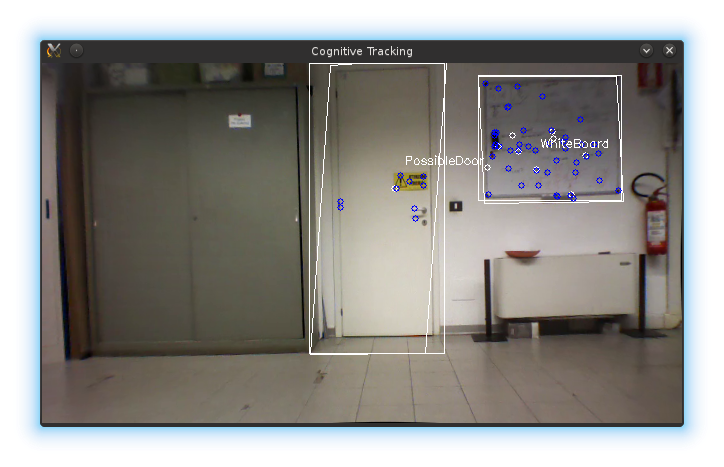
\includegraphics[width=\textwidth]{immagini/risultati/tracker1}
  \caption[Immagine del tracker]{L'algoritmo di riconoscimento ha individuato la lavagna e la porta: esse vengono insegite dal tracker}
  \label{fig:tracker1}
\end{figure}

\begin{figure}[ht]
  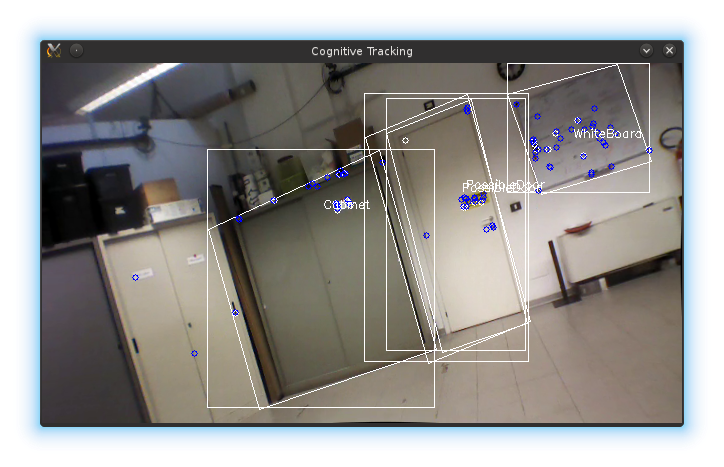
\includegraphics[width=\textwidth]{immagini/risultati/tracker2}
  \caption[Track precedenti da un nuovo punto di vista]{Il tracker mantiene le track riconosciute, e aggiunge la track dell'armadio che ha riconosciuto.}
  \label{fig:tracker2}
\end{figure}